\begin{tikzpicture}
    \node{(1)};
\end{tikzpicture}\;
\begin{tikzpicture}[axpic]
  \begin{scope}[shift={(0.000,0.500)}]
  \pic (g1) at (0.500,0.500) {copy};
  \end{scope}
  \begin{scope}[shift={(1.250,0.000)}]
  \begin{scope}[shift={(0.000,1.000)}]
  \pic (g2) at (0.500,0.500) {ge};
  \end{scope}
  \pic (g3) at (0.500,0.500) {coge};
  \end{scope}
  \draw (g1-out-0) to[out=0,in=180] (g2-in-0);
  \draw (g1-out-1) to[out=0,in=180] (g3-in-0);
  \begin{scope}[shift={(2.500,0.500)}]
  \pic (g4) at (0.500,0.500) {cocopy};
  \end{scope}
  \draw (g2-out-0) to[out=0,in=180] (g4-in-0);
  \draw (g3-out-0) to[out=0,in=180] (g4-in-1);
\end{tikzpicture}
\;\begin{tikzpicture}[axpic]\node{$\subseteq$};\end{tikzpicture}\;
\begin{tikzpicture}[axpic]
  \coordinate (id_in_1) at (0,0.500);
  \coordinate (id_out_2) at (1.000,0.500);
  \draw (id_in_1) -- (id_out_2);
\end{tikzpicture}

\vspace{5mm}

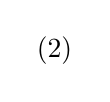
\begin{tikzpicture}
    \node{(2)};
\end{tikzpicture}\;
\begin{tikzpicture}[axpic]
  \coordinate (id_in_1) at (0,0.500);
  \coordinate (id_out_2) at (1.000,0.500);
  \draw (id_in_1) -- (id_out_2);
\end{tikzpicture}
\;\begin{tikzpicture}[axpic]\node{$=$};\end{tikzpicture}\;
\begin{tikzpicture}[axpic]
  \pic (g1) at (0.500,0.500) {copy};
  \begin{scope}[shift={(1.250,0.000)}]
  \pic (g2) at (0.500,0.500) {cocopy};
  \end{scope}
  \draw (g1-out-0) to[out=0,in=180] (g2-in-0);
  \draw (g1-out-1) to[out=0,in=180] (g2-in-1);
\end{tikzpicture}
\;\begin{tikzpicture}[axpic]\node{$\subseteq$};\end{tikzpicture}\;
\begin{tikzpicture}[axpic]
  \begin{scope}[shift={(0.000,0.500)}]
  \pic (g1) at (0.500,0.500) {copy};
  \end{scope}
  \begin{scope}[shift={(1.250,0.000)}]
  \begin{scope}[shift={(0.000,1.000)}]
  \pic (g2) at (0.500,0.500) {ge};
  \end{scope}
  \pic (g3) at (0.500,0.500) {coge};
  \end{scope}
  \draw (g1-out-0) to[out=0,in=180] (g2-in-0);
  \draw (g1-out-1) to[out=0,in=180] (g3-in-0);
  \begin{scope}[shift={(2.500,0.500)}]
  \pic (g4) at (0.500,0.500) {cocopy};
  \end{scope}
  \draw (g2-out-0) to[out=0,in=180] (g4-in-0);
  \draw (g3-out-0) to[out=0,in=180] (g4-in-1);
\end{tikzpicture}

\vspace{5mm}
\;\begin{tikzpicture}[axpic]\node{$(1)\wedge(2)\implies$};\end{tikzpicture}\;
\begin{tikzpicture}[axpic]
  \coordinate (id_in_1) at (0,0.500);
  \coordinate (id_out_2) at (1.000,0.500);
  \draw (id_in_1) -- (id_out_2);
\end{tikzpicture}
\;\begin{tikzpicture}[axpic]\node{$=$};\end{tikzpicture}\;
\begin{tikzpicture}[axpic]
  \begin{scope}[shift={(0.000,0.500)}]
  \pic (g1) at (0.500,0.500) {copy};
  \end{scope}
  \begin{scope}[shift={(1.250,0.000)}]
  \begin{scope}[shift={(0.000,1.000)}]
  \pic (g2) at (0.500,0.500) {ge};
  \end{scope}
  \pic (g3) at (0.500,0.500) {coge};
  \end{scope}
  \draw (g1-out-0) to[out=0,in=180] (g2-in-0);
  \draw (g1-out-1) to[out=0,in=180] (g3-in-0);
  \begin{scope}[shift={(2.500,0.500)}]
  \pic (g4) at (0.500,0.500) {cocopy};
  \end{scope}
  \draw (g2-out-0) to[out=0,in=180] (g4-in-0);
  \draw (g3-out-0) to[out=0,in=180] (g4-in-1);
\end{tikzpicture}
